%fiber_modeling

%fiber_modeling.tex
First agenda is to determine the Tapered and Lensed Fiber (TLF) model. Because of the heave computing cost creating a full size fiber is not economical. Therefore only the end of the fiber, which provides approximately the equal technical properties, will be modeled in this works.  In \cite{TLF_analysis,TLF_mode_transforming} two type of the TLF configuration are mentioned. 


\begin{figure}[!ht]
\centering
\subfigure[Tapered cladding TLF.]{
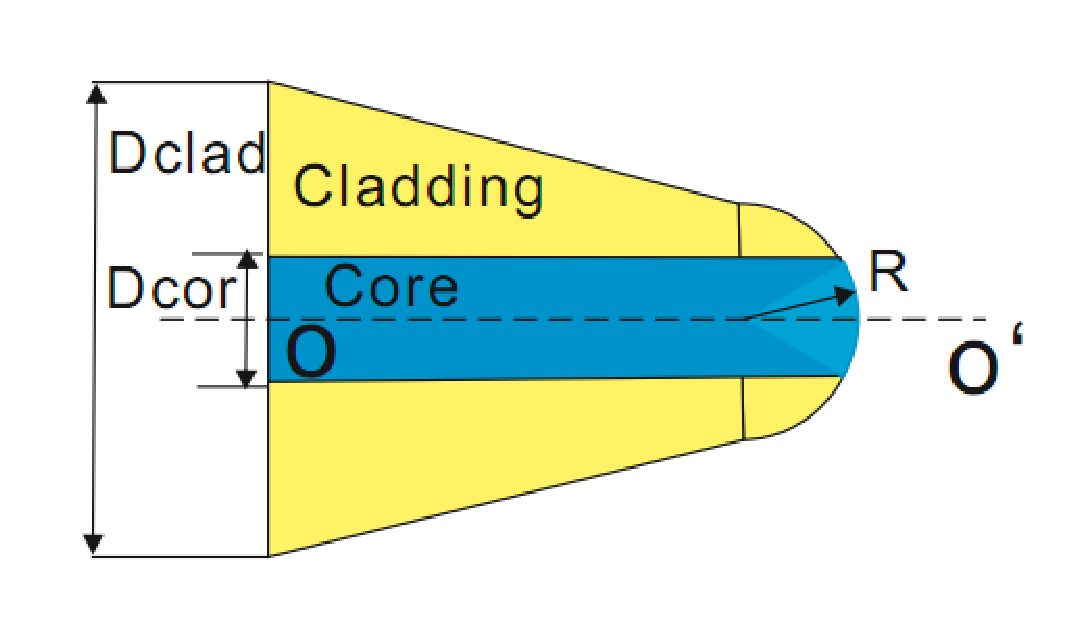
\includegraphics[width=0.4\textwidth]{bilder/lense_fiber_01}
\label{fig:lense_fiber_01}
}
\hfill
\subfigure[Tapered core TLF.]{
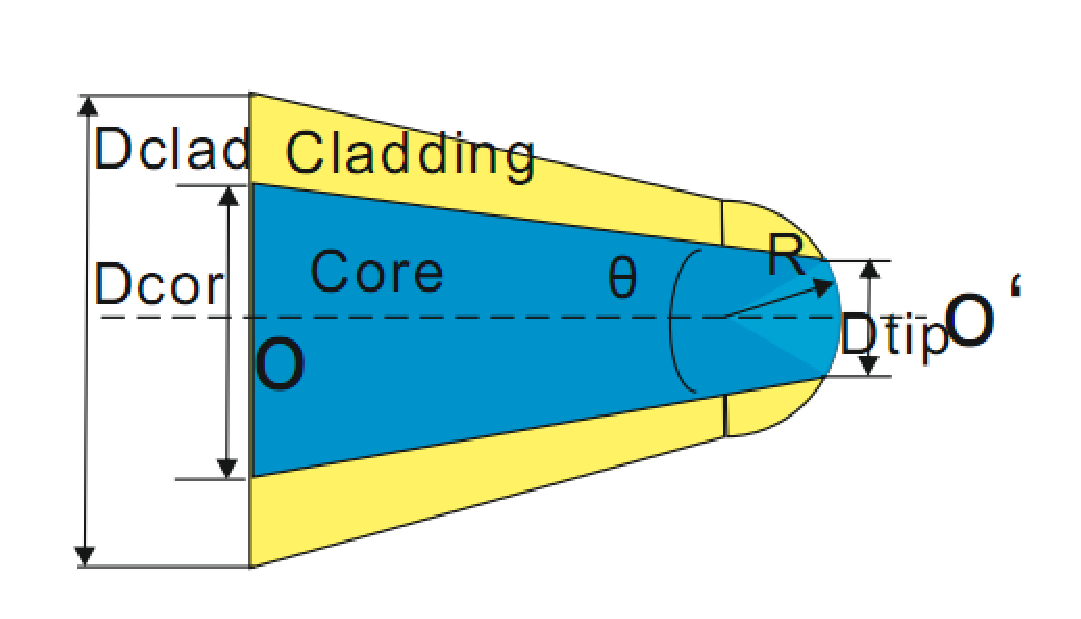
\includegraphics[width=0.4\textwidth]{bilder/lense_fiber_02}
\label{fig:lense_fiber_02}
}
\label{fig:two_TLF}
\caption{Two types of Tapered and Lensed Fibers}
\end{figure}

The tapered cladding TLF Fig.\quad\ref{fig:lense_fiber_01} shows that its cladding diameter decreases along the beam propagation direction (O-O'Axis) and its core diameter is a constant. For the tapered core TLF Fig.\quad\ref{fig:lense_fiber_02} its cladding diameter and core diameter both decrease along the axis. In \cite{TLF_mode_transforming} the Authour tried to develop methods to estimate the performance of both type of TLF. His results show that the performance of the first type of TLF agrees well with the estimation and that of the second type is unpredictable. In this section two TLF models from each type are created and their performances are tested in CST MWS.  
First of all, determination the lens of both types is primary. For simplification, a hemispherical lens is assumed at the end of the fiber. Considering the working distance of the practical TLF, the lens configuration can be estimated through the lens theory. After estimations and some simulations one configuration of the lens is carefully selected Tab.\quad\ref{tab:model_fiber_configuration}.   

\begin{table}
\caption{Configurations of the TLF Models}
\centering
\begin{tabular}{ccc}
\hline
							&Tapered Cladding&Tapered Core\\
\hline
R($\mu$m) & $6$						 &$6$	\\
n$_{core}$&$1.68$&$1.68$\\
n$_{cladding}$&$1.66$&$1.66$\\
D$_{clad}$($\mu$m) &	$17$ &	$17$\\
D$_{core}$($\mu$m) & $10$ &	$17$\\
D$_{tip}$ ($\mu$m) & --   &	$6$\\
\hline
\end{tabular}
\label{tab:model_fiber_configuration}
\end{table}
From Fig.\quad\ref{fig:lens_spot} the beam propagation is demonstrated base on lens theory. As is in previous chapter described, the minimum spot located not exactly at the focal length. From measures of the location of Paraxial focal plane(PP) and that of meridional plane (MP) the minimum spot(MS) can be estimated. In the above configuration the theoretical distance from lens end to PP is $8.82 \mu$ m and the distance from lens end to MP is about $2.74 \mu$m. Backword $3/4$ longitudinal spherical aberration(LAm) form PP, the MS is founded at the place about $4.26 \mu$m far from lens end. 
\begin{figure}[!ht]
\centering
	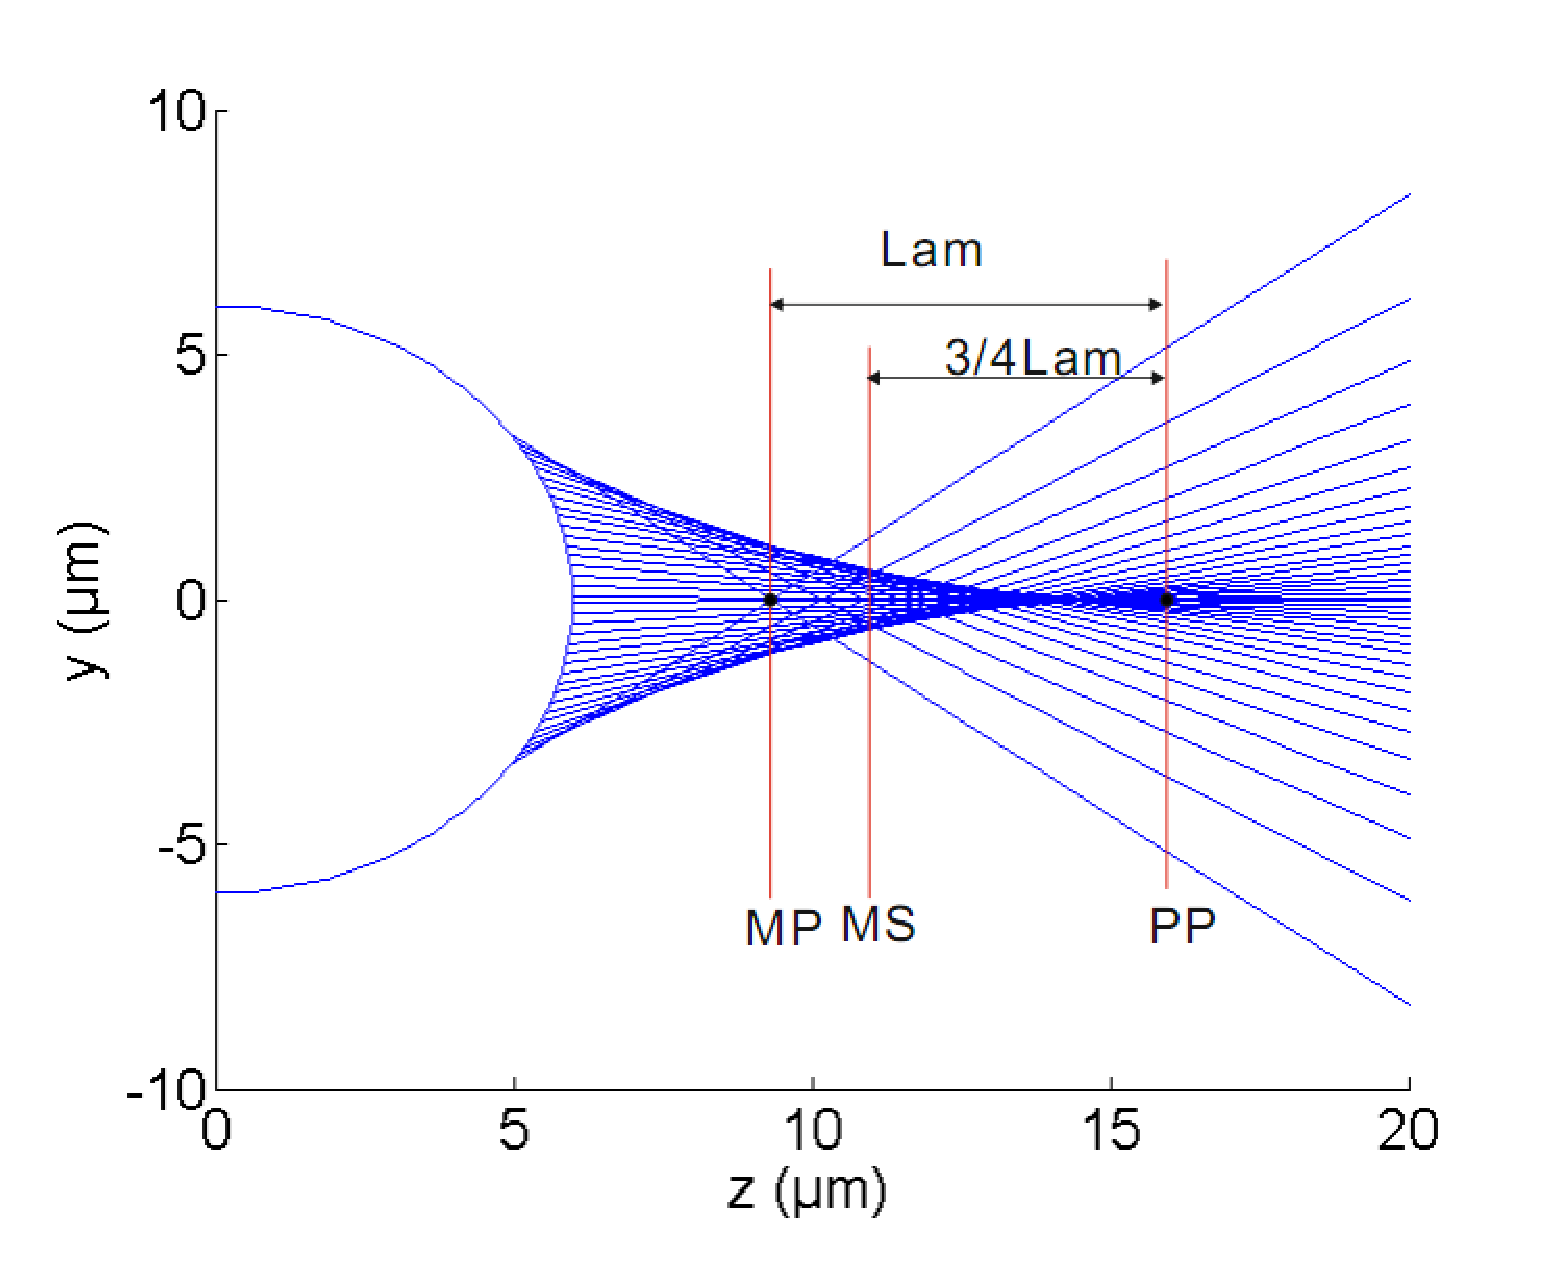
\includegraphics[width=0.7\textwidth]{bilder/cal_min_spot}
\caption{Beam Propogation from lense.}
\label{fig:lens_spot}
\end{figure}
Implement this configuration for both types of TLF models in CST. Through simulations, E-Field demonstrations in the xz-plane of both types of TLFs can be drown as Fig. \ref{fig:Tapered_cladding_efield} and  Fig. \ref{fig:Tapered_core_efield}, wich have no great difference.
\begin{figure}[!ht]
	\centering
		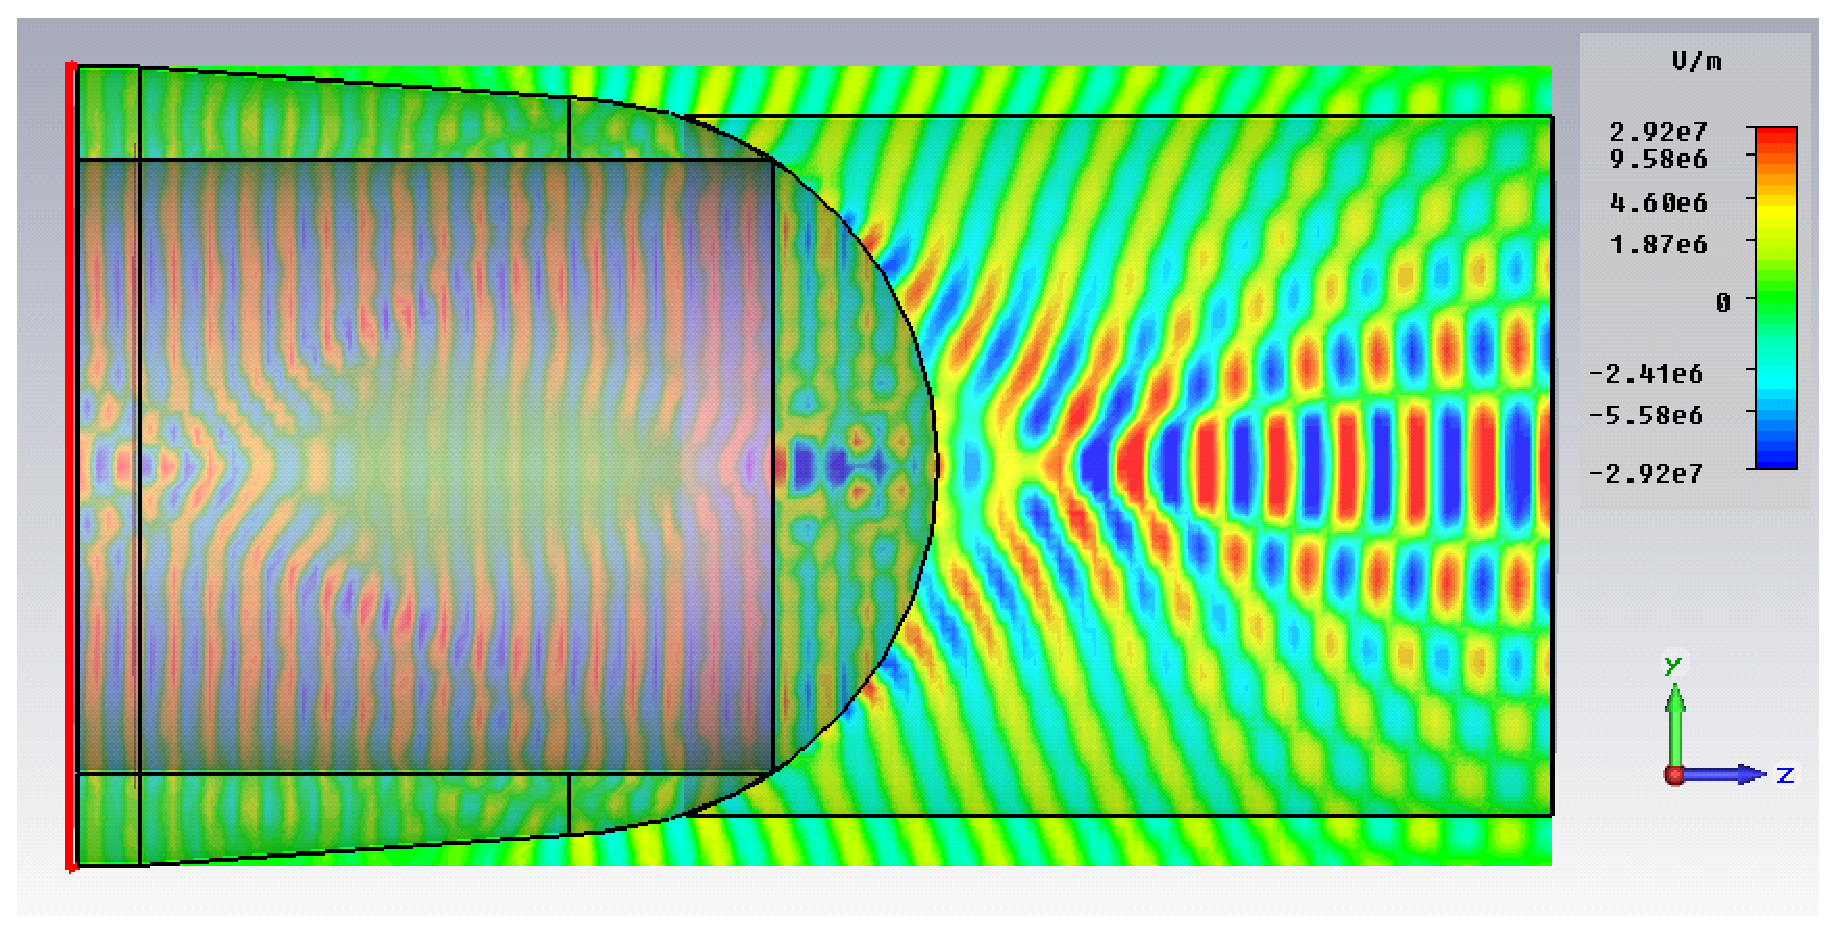
\includegraphics[width=0.8 \textwidth]{bilder/cst_lensed_fiber_equ_efield}
		\caption{E-Field demonstration of Tapered cladding TLF}
 		\label{fig:Tapered_cladding_efield}
\end{figure}

\begin{figure}[!ht]
	\centering
		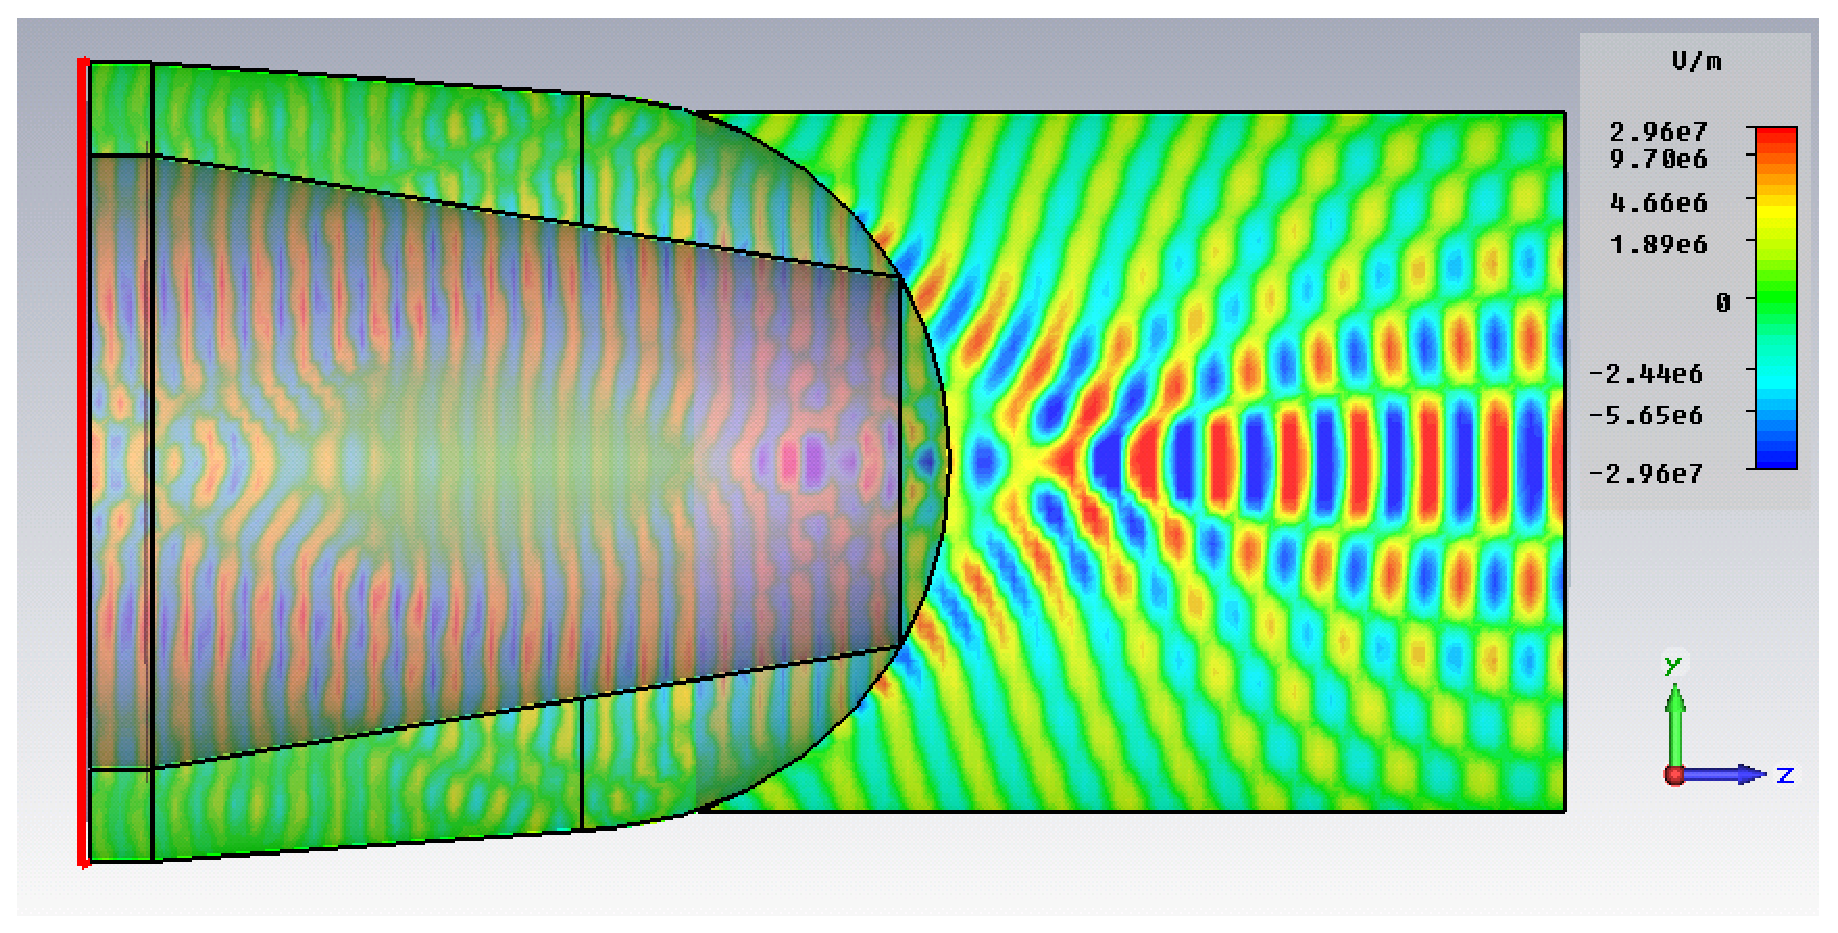
\includegraphics[width=0.8 \textwidth]{bilder/cst_lensed_fiber_efield}
		\caption{E-Field demonstration of Tapered core TLF}
 		\label{fig:Tapered_core_efield}	
\end{figure}
Load the its beam propagation detail into Matlab workspace and draw
Fig.\ref{fig:Tapered_cladding_spot_curve} and Fig.\ref{fig:Tapered_core_spot_curve},which shows the beam spot diameters through their absolute beam power flow densities or its z-compents(propagation direction) along the propagation distance. From these two figures, curves of the absolute value of their power flow density are more obvious to help people to find the minimum spot of lenses. In Fig.\ref{fig:Tapered_cladding_spot_curve} that the minimum spot size locate at about $4.1 \mu m$ from lense end and spot size equal about $1.5 \mu m$. While in Fig.\ref{fig:Tapered_core_spot_curve} that the minimum spot size is found at  $4.3 \mu m$ from lense end and spot size equal about $1.5 \mu m$. Thus it is concluded that two configuration has only a small difference. By rechecking the properties in Tab.\ref{tab:technical parameters_lensed_fiber} both TLF model are acceptable for the following development. In this works the tapered core TLF will be used for further simulations.
Fig.\ref{fig:Tapered_cladding_spot_curve}-\ref{fig:Tapered_core_spot_curve} to illustrate the beam Spot size diameter along the longitude axis.
\begin{figure}[!ht]
		\centering
		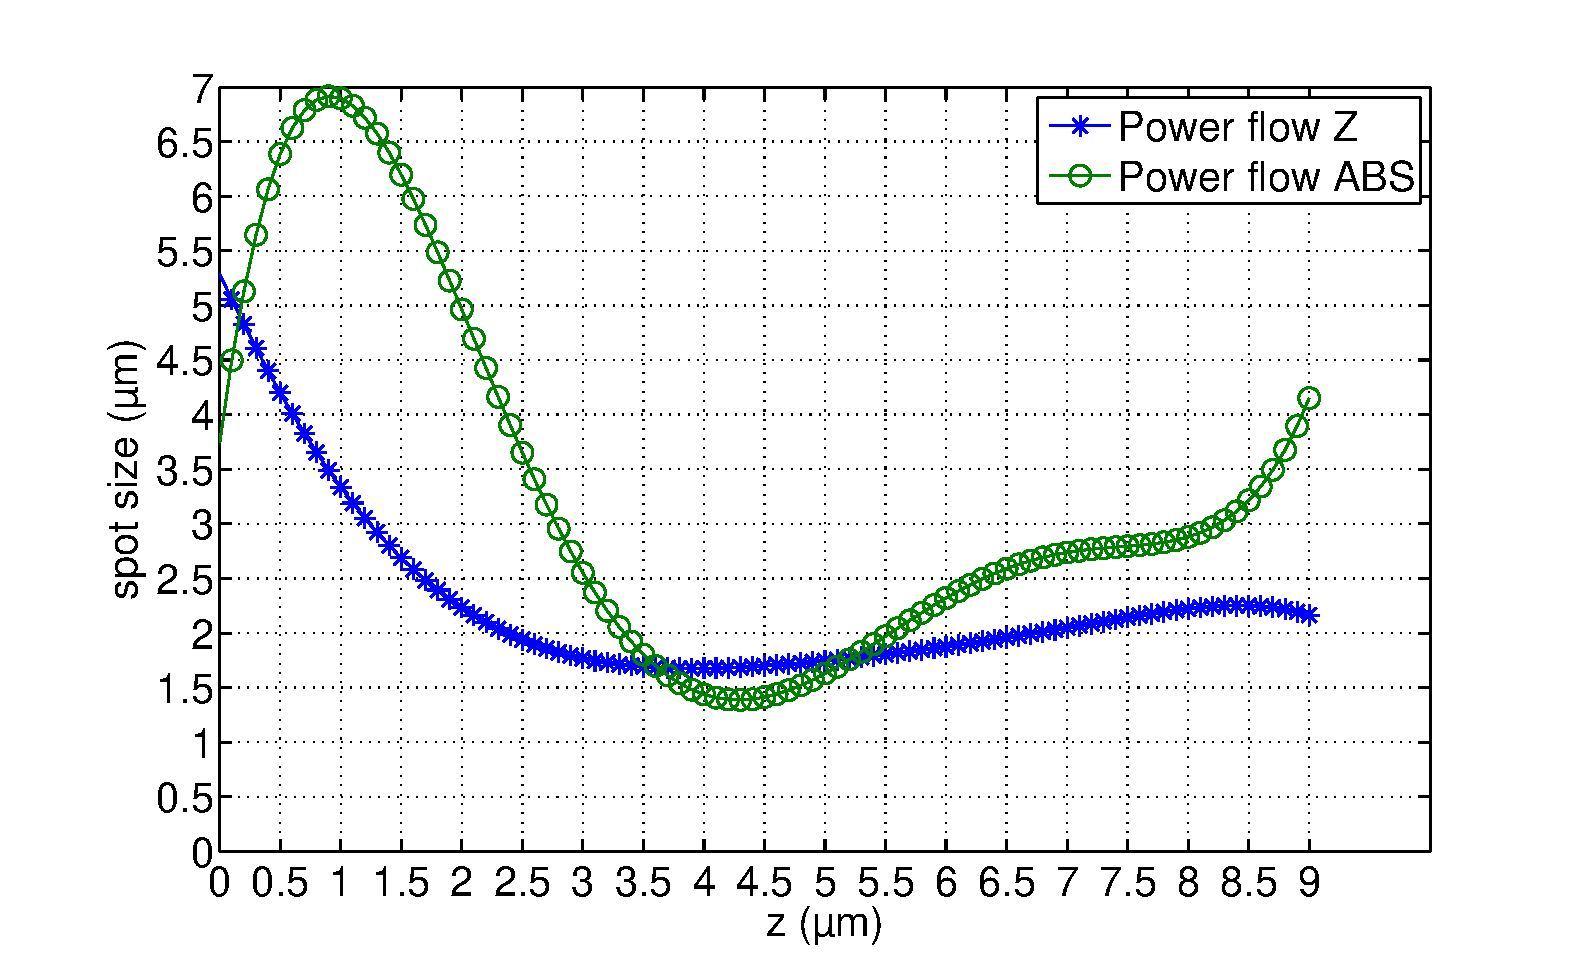
\includegraphics[width=0.7 \textwidth]{bilder/Tapered_cladding_spot_curve}
		\caption{Spot Size Curve of Tapered cladding TLF}
		\label{fig:Tapered_cladding_spot_curve}
\end{figure} 
\begin{figure}[!ht]
		\centering
		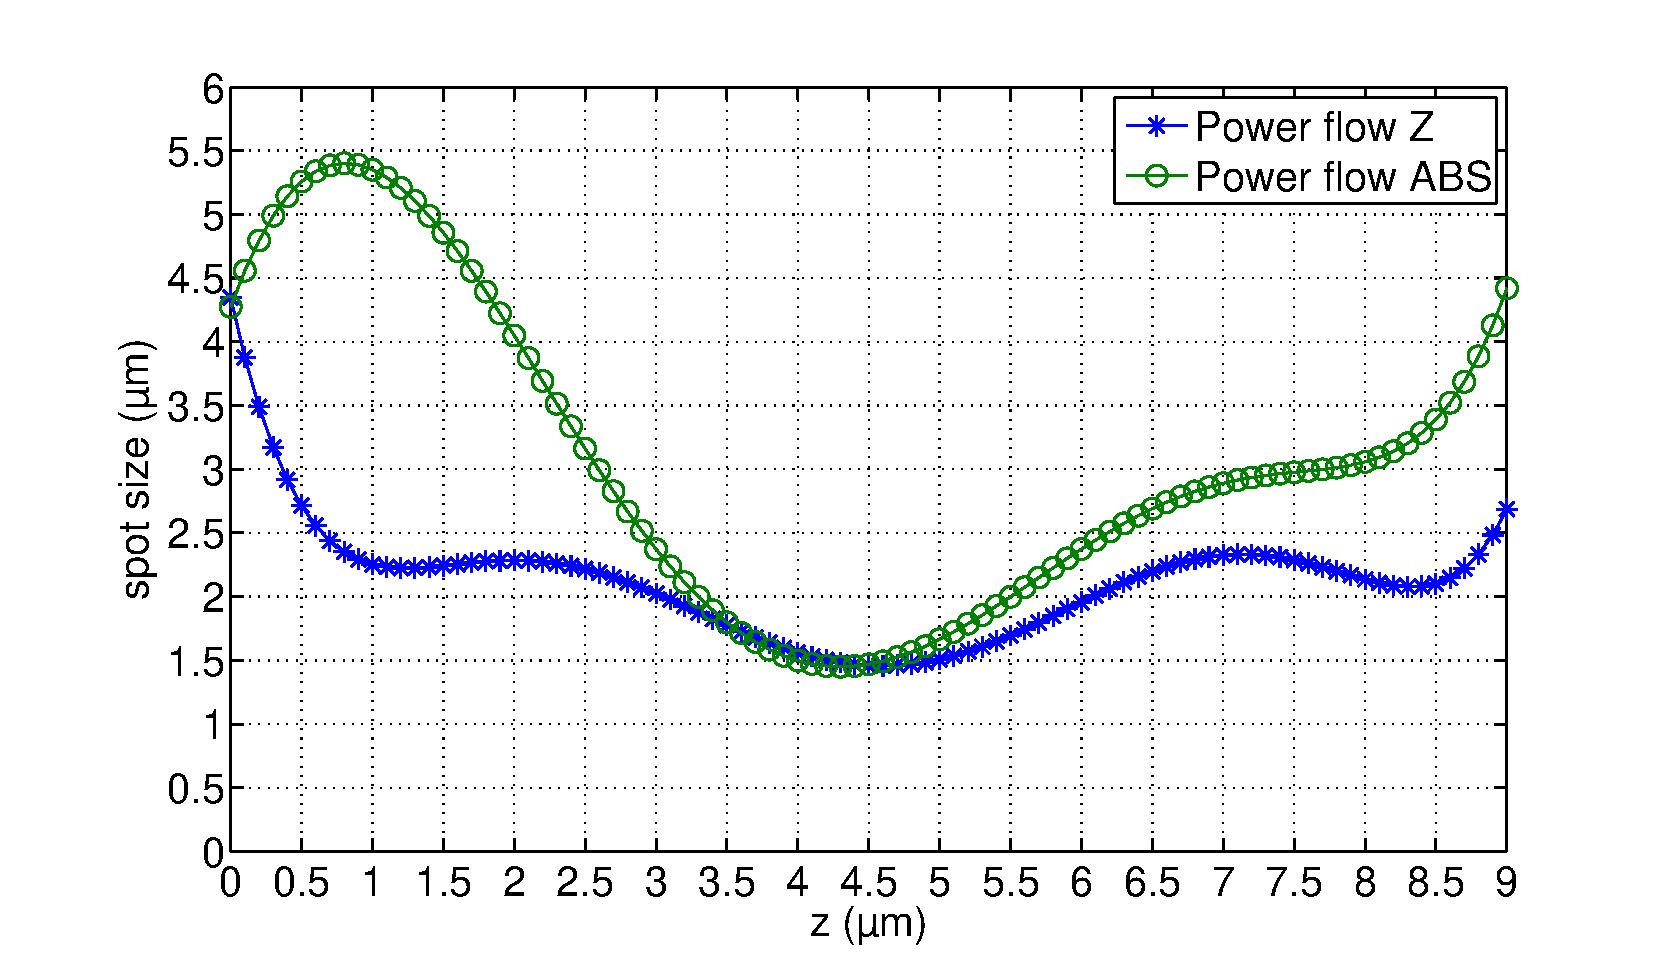
\includegraphics[width=0.7 \textwidth]{bilder/Tapered_core_spot_curve}
		\caption{Spot Size Curve of Tapered core TLF}
 		\label{fig:Tapered_core_spot_curve}	
\end{figure}

For a clear view of the beam propagation from the tapered core TLF, 3D Fig.\quad\ref{fig:3d_spot_sub1}-\ref{fig:3d_spot_sub8} of beam power densities at different distances are demonstrated. It is obvious that the power density of the beam center rise firstly along the distance and at $4\mu$m reach the hightest value. Then it falls slowly. This tendency agrees with its spot size curve inversely. 
\begin{figure}[!ht]
\setlength{\abovecaptionskip}{0pt}% 
\flushleft
	\subfigure[3D Beam Power at distance $1\mu m$]{
	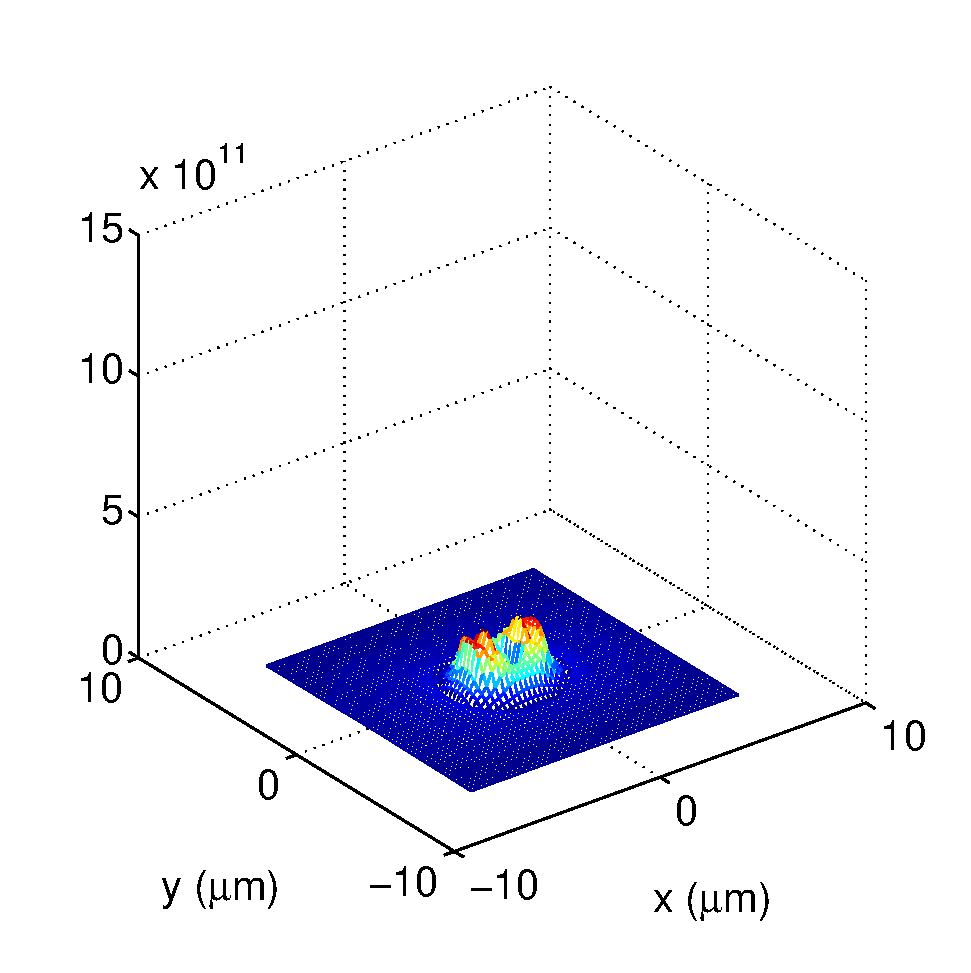
\includegraphics[width=0.4 \textwidth]{bilder/surf_spot_1um}
	\label{fig:3d_spot_sub1}%
	}
 	\subfigure[3D Beam Power at distance $2\mu m$]{
 	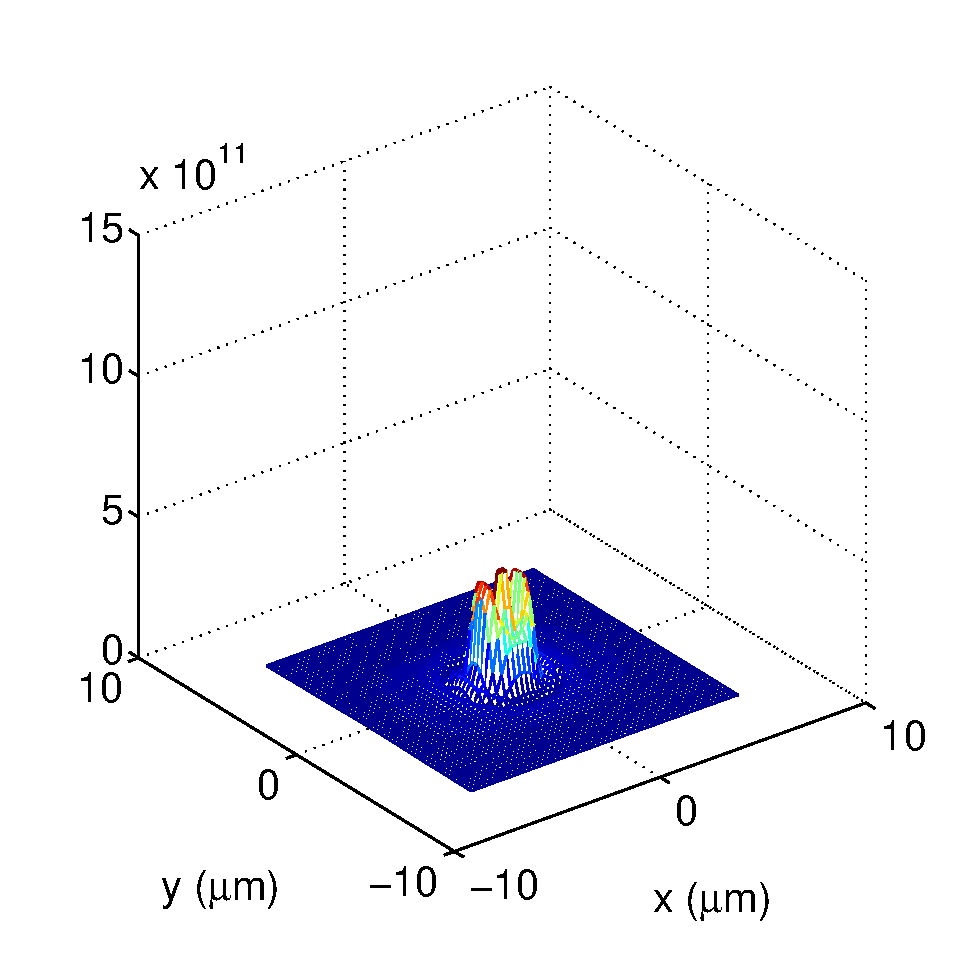
\includegraphics[width=0.4 \textwidth]{bilder/surf_spot_2um}
 	\label{fig:3d_spot_sub2}
 	}
\end{figure}	
\begin{figure}[!ht]
\setlength{\abovecaptionskip}{0pt}% 
\flushleft
 	 	\subfigure[3D Beam Power at distance $3\mu m$]{
 	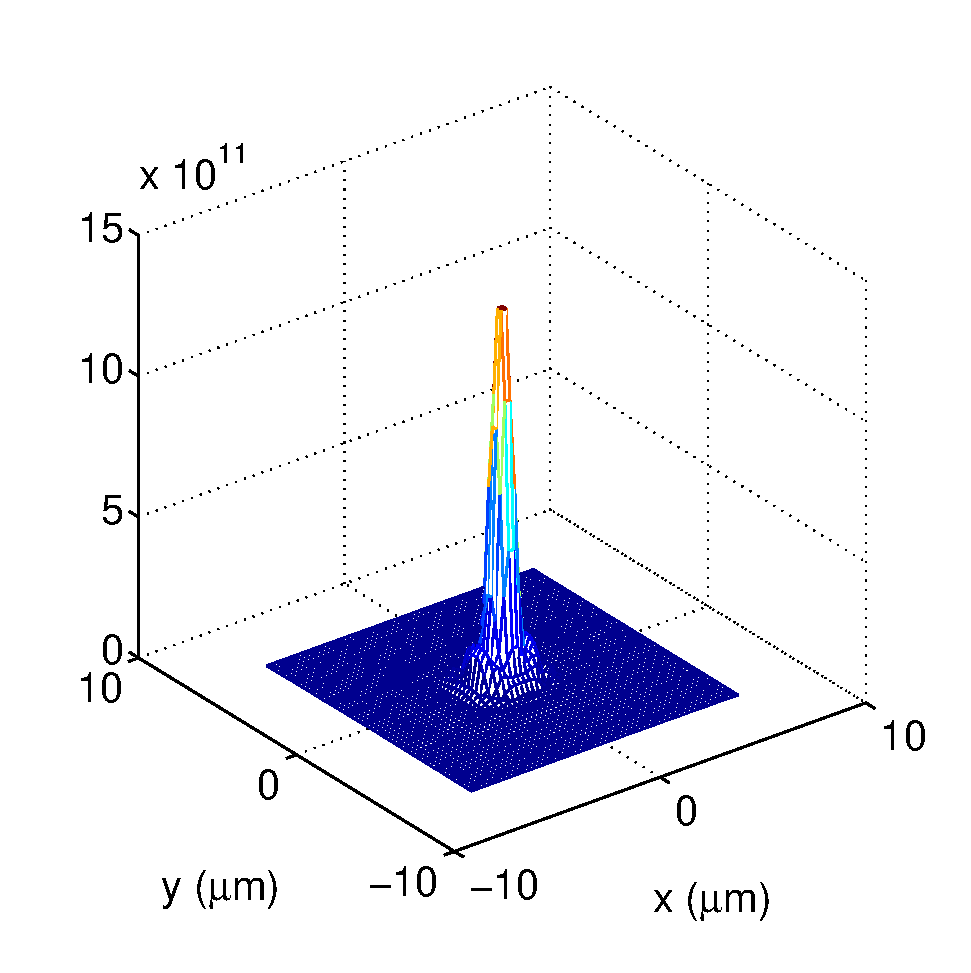
\includegraphics[width=0.4 \textwidth]{bilder/surf_spot_3um}
 	\label{fig:3d_spot_sub3}
 	}
 	\subfigure[3D Beam Power at distance $4\mu m$]{
 	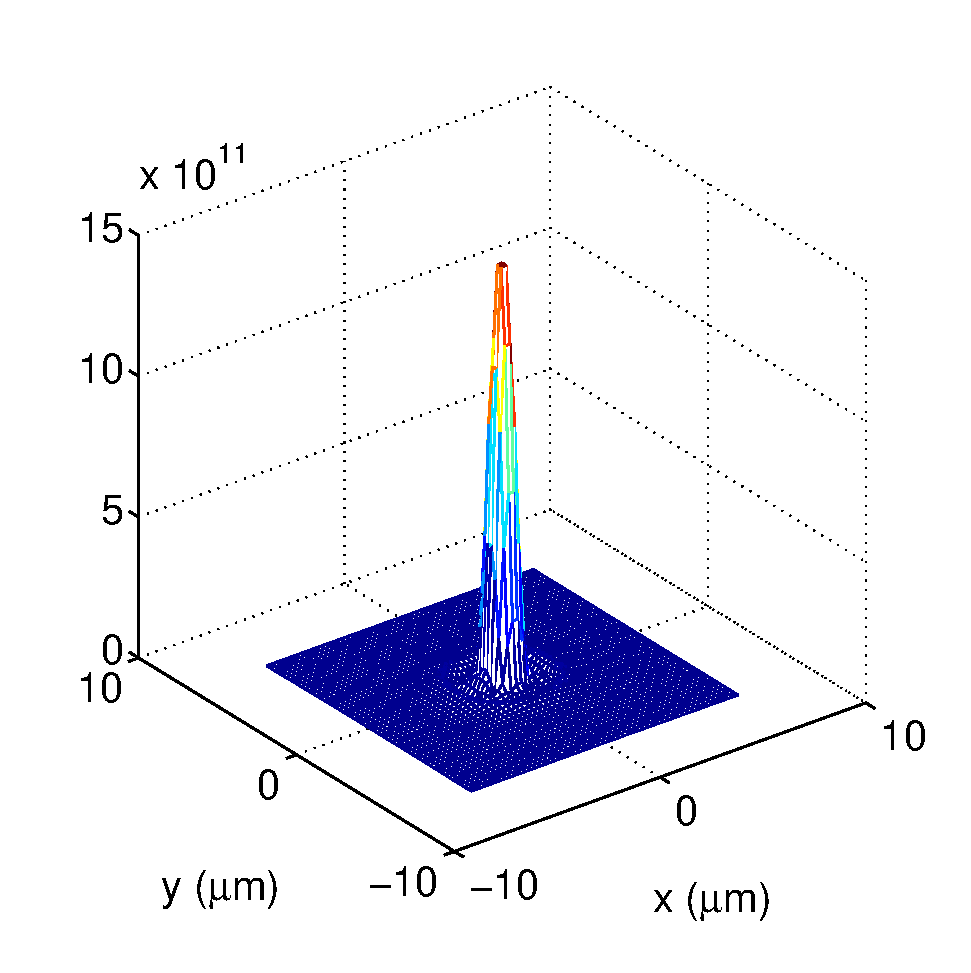
\includegraphics[width=0.4 \textwidth]{bilder/surf_spot_4um}
 	\label{fig:3d_spot_sub4}
 	}
\end{figure}	
\begin{figure}[!ht]
\setlength{\abovecaptionskip}{0pt}% 
\flushleft
 	 \subfigure[3D Beam Power at distance $5\mu m$]{
 	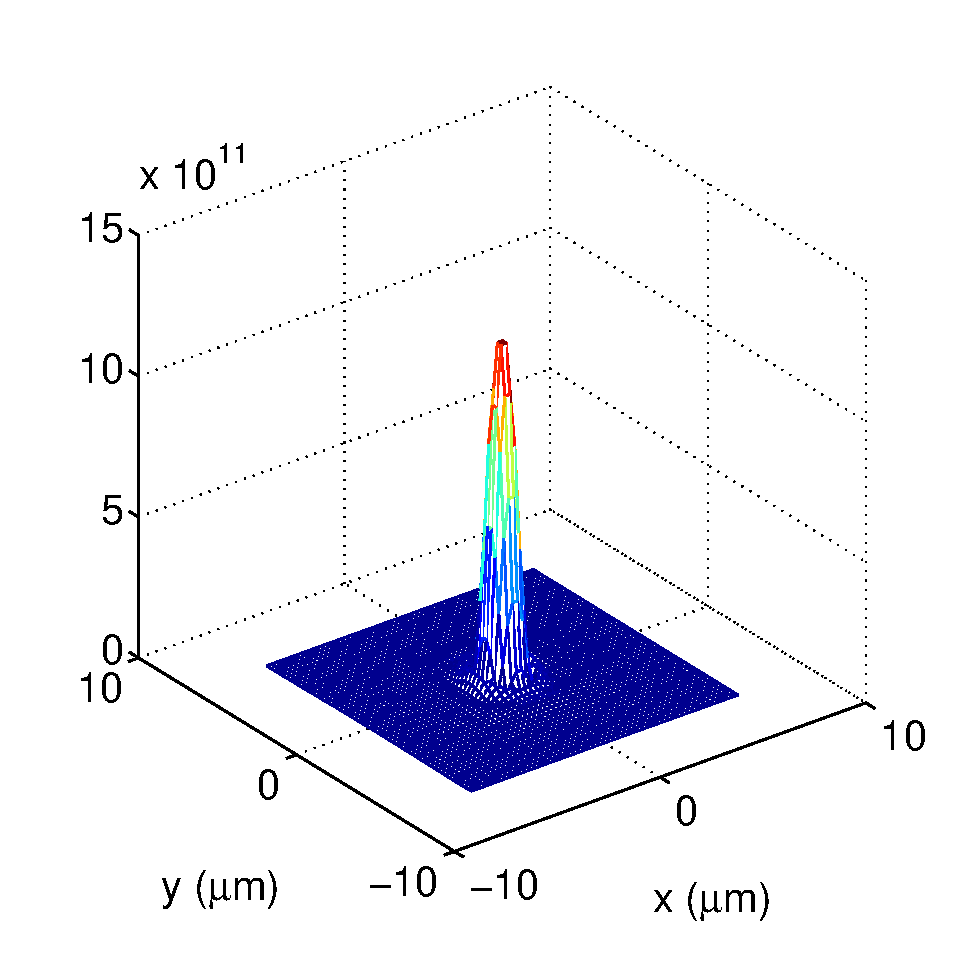
\includegraphics[width=0.4 \textwidth]{bilder/surf_spot_5um}
 	\label{fig:3d_spot_sub5}
 	}
 	 	\subfigure[3D Beam Power at distance $6\mu m$]{
 	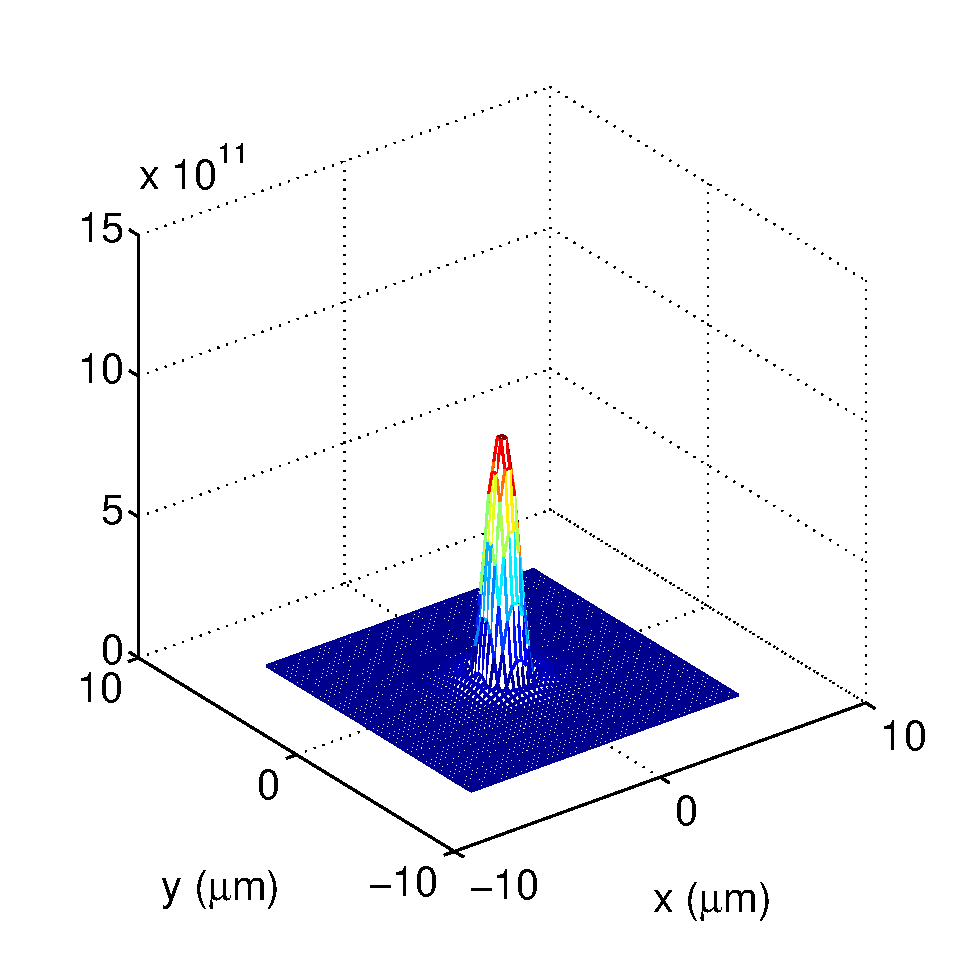
\includegraphics[width=0.4 \textwidth]{bilder/surf_spot_6um}
 	\label{fig:3d_spot_sub6}
 	}
\end{figure}	
\begin{figure}[!htp]
\setlength{\abovecaptionskip}{0pt}% 
\flushleft
  \subfigure[3D Beam Power at distance $7\mu m$]{
 	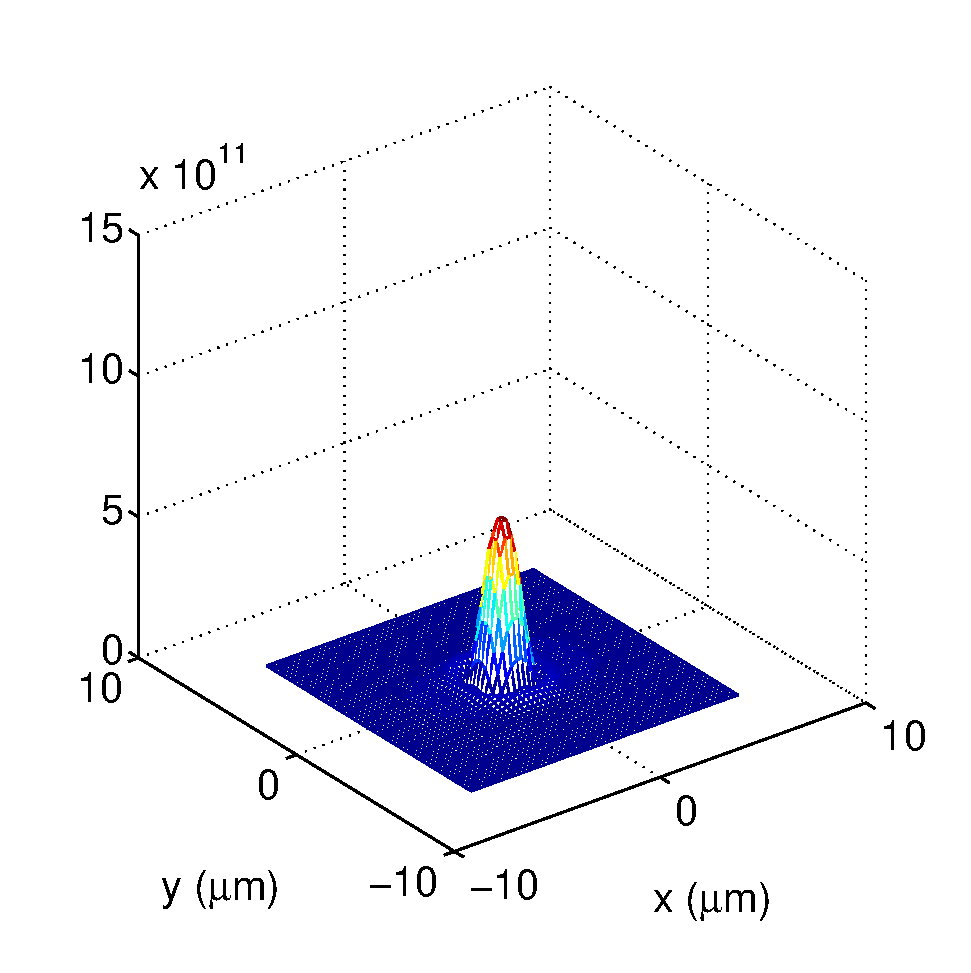
\includegraphics[width=0.4 \textwidth]{bilder/surf_spot_7um}
 	\label{fig:3d_spot_sub7}
 	}
 	\subfigure[3D Beam Power at distance $8\mu m$]{
 	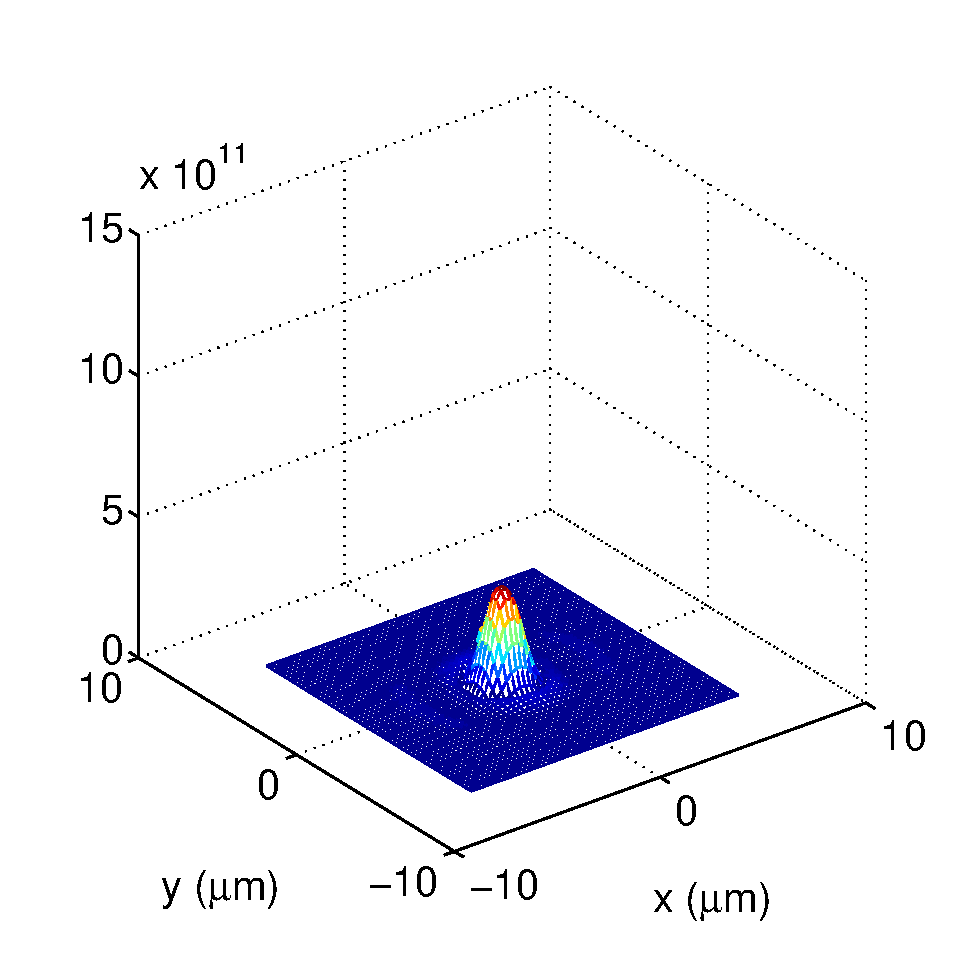
\includegraphics[width=0.4 \textwidth]{bilder/surf_spot_8um}
 	\label{fig:3d_spot_sub8}
 	}
 	\caption{3D Beam Power }
\end{figure} 
